\documentclass[11pt]{article} 
\usepackage[english]{babel}
\usepackage[utf8]{inputenc}
\usepackage[margin=0.5in]{geometry}
\usepackage{amsmath}
\usepackage{amsthm}
\usepackage{amsfonts}
\usepackage{amssymb}
\usepackage[usenames,dvipsnames]{xcolor}
\usepackage{graphicx}
\usepackage[siunitx]{circuitikz}
\usepackage{tikz}
\usepackage[colorinlistoftodos, color=orange!50]{todonotes}
\usepackage{hyperref}
\usepackage[numbers, square]{natbib}
\usepackage{fancybox}
\usepackage{epsfig}
\usepackage{soul}
\usepackage[framemethod=tikz]{mdframed}
\usepackage[shortlabels]{enumitem}
\usepackage[version=4]{mhchem}
\usepackage{multicol}
\usepackage{forest}
\usepackage{mathtools}
\usepackage{comment}
\usepackage{enumitem}
\usepackage[utf8]{inputenc}
\usepackage[linesnumbered,ruled,vlined]{algorithm2e}
\usepackage{listings}
\usepackage{color}
\usepackage[numbers]{natbib}
\usepackage{subfiles}
\usepackage{tkz-berge}
\usepackage{fancyvrb}
\lstset{
basicstyle=\small\ttfamily,
columns=flexible,
breaklines=true
}



\newtheorem{prop}{Proposition}[section]
\newtheorem{thm}{Theorem}[section]
\newtheorem{lemma}{Lemma}[section]
\newtheorem{cor}{Corollary}[prop]

\theoremstyle{definition}
\newtheorem{definition}{Definition}

\theoremstyle{definition}
\newtheorem{required}{Problem}
\newtheorem*{requiredHC}{Problem HC}

\theoremstyle{definition}
\newtheorem{ex}{Example}


\setlength{\marginparwidth}{3.4cm}
%#########################################################

%To use symbols for footnotes
\renewcommand*{\thefootnote}{\fnsymbol{footnote}}
%To change footnotes back to numbers uncomment the following line
%\renewcommand*{\thefootnote}{\arabic{footnote}}

% Enable this command to adjust line spacing for inline math equations.
% \everymath{\displaystyle}

% _______ _____ _______ _      ______ 
%|__   __|_   _|__   __| |    |  ____|
%   | |    | |    | |  | |    | |__   
%   | |    | |    | |  | |    |  __|  
%   | |   _| |_   | |  | |____| |____ 
%   |_|  |_____|  |_|  |______|______|
%%%%%%%%%%%%%%%%%%%%%%%%%%%%%%%%%%%%%%%

\title{
\normalfont \normalsize 
\textsc{CSCI 3104 Fall 2022 \\ 
Instructors: Prof. Grochow and Candra Kanth Nagesh} \\
[10pt] 
\rule{\linewidth}{0.5pt} \\[6pt] 
\huge Problem Set 1 \\
\rule{\linewidth}{2pt}  \\[10pt]
}
%\author{}
\date{}

\begin{document}

\maketitle


%%%%%%%%%%%%%%%%%%%%%%%%%
%%%%%%%%%%%%%%%%%%%%%%%%%%
%%%%%%%%%%FILL IN YOUR NAME%%%%%%%
%%%%%%%%%%AND STUDENT ID%%%%%%%%
%%%%%%%%%%%%%%%%%%%%%%%%%%
\noindent
Due Date \dotfill September 5, 2022  \\
Name \dotfill \textbf{Tyler Huynh} \\
Student ID \dotfill \textbf{109603994} \\
Collaborators \dotfill \textbf{No Collaborators}

\tableofcontents

\section*{Instructions}
\addcontentsline{toc}{section}{Instructions}
 \begin{itemize}
	\item The solutions \textbf{should be typed}, using proper mathematical notation. We cannot accept hand-written solutions. \href{http://ece.uprm.edu/~caceros/latex/introduction.pdf}{Here's a short intro to \LaTeX.}
	\item You should submit your work through the \textbf{class Gradescope page} only (linked from Canvas). Please submit one PDF file, compiled using this \LaTeX \ template.
	\item You may not need a full page for your solutions; pagebreaks are there to help Gradescope automatically find where each problem is. Even if you do not attempt every problem, please submit this document with no fewer pages than the blank template (or Gradescope has issues with it).

	\item You are welcome and encouraged to collaborate with your classmates, as well as consult outside resources. You must \textbf{cite your sources in this document.} \textbf{Copying from any source is an Honor Code violation. Furthermore, all submissions must be in your own words and reflect your understanding of the material.} If there is any confusion about this policy, it is your responsibility to clarify before the due date. 

	\item Posting to \textbf{any} service including, but not limited to Chegg, Reddit, StackExchange, etc., for help on an assignment is a violation of the Honor Code.

	\item You \textbf{must} virtually sign the Honor Code (see Section \ref{HonorCode}). Failure to do so will result in your assignment not being graded.
\end{itemize}


\section*{Honor Code (Make Sure to Virtually Sign)} \label{HonorCode}
\addcontentsline{toc}{section}{Honor Code (Make Sure to Virtually Sign)}

\begin{requiredHC}
\begin{itemize}
\item My submission is in my own words and reflects my understanding of the material.
\item Any collaborations and external sources have been clearly cited in this document.
\item I have not posted to external services including, but not limited to Chegg, Reddit, StackExchange, etc.
\item I have neither copied nor provided others solutions they can copy.
\end{itemize}

%\noindent In the specified region below, clearly indicate that you have upheld the Honor Code. Then type your name. 
\end{requiredHC}

\begin{proof}[I agree to the above, Tyler Huynh.]
%% Typing "I agree to the above," followed by your name is sufficient.
\end{proof}


\newpage
\section{Standard 1: Proof by Induction}

\subsection{Problem \ref{Induction1}}
\begin{required} \label{Induction1}
A student is trying to prove by induction that $2^{n} < n!$ for $n \geq 4$. 

\begin{proof}[Student's Proof]
The proof is by induction on $n \geq 4$. 
\begin{itemize}
\item \textbf{Base Case:} When $n = 4$, we have that:
\begin{align*}
2^{4} &= 16 \\
&\leq 24 \\
&= 4!
\end{align*}

\item \textbf{Inductive Hypothesis:} Now suppose that for all $k \geq 6$ we have that $2^{k} < k!$. 

\item \textbf{Inductive Step:} We now consider the $k+1$ case. As $k+1 > 6$, we have from the inductive hypothesis that $2^{k+1} < (k+1)!$. The result follows by induction.
\end{itemize}
\end{proof}

There are two errors in this proof. 
\begin{enumerate}[label=(\alph*)]
\item The Inductive Hypothesis is not correct. Write an explanation to the student explaining why their Inductive Hypothesis is not correct. [\textbf{Note:} You are being asked to explain why the Inductive Hypothesis is wrong, and \textbf{not} to rewrite a corrected Inductive Hypothesis.]


\begin{proof}[Answer]
Their inductive hypotheses is not correct because they assume that all values of k  $\ge$ 6, such that $2^k$ $< $ k!. This is not correct because they cannot assume that for the values of k that are greater than or equal to 6 it will prove their hypothesis as being correct, as they are assuming what they are trying to prove.
\end{proof}



\vskip 15pt
\item The Inductive Step is not correct. Write an explanation to the student explaining why their Inductive Step is not correct. [\textbf{Note:} You are being asked to explain why the Inductive Step is wrong, and \textbf{not} to rewrite a corrected Inductive Step.]

\begin{proof}[Answer]
The inductive step is not correct because the student is assuming that $k + 1 > 6$, such that $2^k+1$ $<$ $(k+1)!$. This is incorrect due to the fact that they don't provide any steps on how to prove that they reached this conclusion.This concludes that their inductive hypothesis is incorrect leading to their inductive step also being incorrect.
\end{proof}
\end{enumerate}
\end{required}





\newpage
\subsection{Problem \ref{Induction2}} 
\begin{required} \label{Induction2}
Consider the recurrence relation, defined as follows:
\[
T_{n} = \begin{cases} 2 & : n = 0, \\
22 & : n = 1, \\
-2 T_{n-1} + 35 T_{n-2} & : n \geq 2.
\end{cases}
\]

\noindent Prove by induction that $T_{n} = (-1) \cdot (-7)^{n} + 3 \cdot (5)^{n}$, for all integers $n \in \mathbb{N}$. [\textbf{Recall:} $\mathbb{N} = \{0, 1, 2, \ldots \}$ is the set of non-negative integers.]
\end{required}

\begin{proof} \textbf{Proof by Strong Induction.}\\\\
\textbf {Base Case:} \\ 
When \\
\indent $n = 0$ then $T_0 = 2$, we have that:\\ 
\indent\indent$T_0 = (-1)*(-7)^0 + 3*(5)^0$ \\
\indent\indent\indent= -1 + 3 \\
\indent\indent\indent2 = 2 \\
\indent $n = 1$ then $T_1 = 22$, we have that: \\
\indent\indent$T_1 = (-1)*(-7)^1 + 3*(5)^1$\\
\indent\indent= 7+15 \\
\indent\indent\indent22 = 22\\

\textbf{Inductive Hypothesis:} \\

For n $\ge$ 2, such that $k < n$ $T_k = (-1)*(-7)^k + 3*(5)^k$, such that our recurrence relation: \\
\indent $-2T_{k-1} + 35T_{k-2} = (-1)*(-7)^k + 3*(5)^k$, will stand true.\\

\textbf{Inductive Step:}\\
We know that by the inductive hypothesis, that $k < n$, such that: \\
\indent $n-1 < n$ and $n-2 < n$ \\
Plugging this into $T_n$: \\
\indent$T_{n-1} = (-1) * (-7)^{n-1} + 3 * (5)^{n-1}$\\
\indent$T_{n-2} = (-1) * (-7)^{n-2} + 3 * (5)^{n-2}$ \\
Further by our inductive hypothesis we know that: \\ 
\indent$T_n = -2T_{k-1} + 35T_{k-2}$ \\
So plugging in previously: \\
\indent $T_n = -2(-1*(-7)^{n-1} + 3*(5)^{n-1}) + 35(-1*(-7)^{n-2} + 3*(5)^{n-2})$\\
Solving for this: \\
\indent$T_n = ((2*(-7)^{n-1} - 6*(5)^{n-1}) + (-35*(-7)^{n-2} + 105*(5)^{n-2}))$ \\
\indent $T_n = ((-\frac{2}{7}(-7)^n + -\frac {6}{5}(5)^n) + (-\frac{35}{49}(-7)^n + \frac{105}{25}(5)^n))$ \\
\indent  $T_n = ((-\frac{2}{7}(-7)^n + -\frac {6}{5}(5)^n) + (-\frac{5}{7}(-7)^n + \frac{21}{5}(5)^n))$ \\
\indent $T_n = ((-\frac{2}{7}(-7)^n  - \frac{5}{7}(-7)^n) + (-\frac {6}{5}(5)^n + \frac{21}{5}(5)^n))$ \\
\indent $T_n = ((-1(-7)^n + 3(5)^n))$ \\
Thus, as you can see from the above work, we can see that that $T_{n} = (-1) * (-7)^{n} + 3 * (5)^{n}$, for all integers $n \in \mathbb{N}$ has been proved by using strong induction.
\end{proof}



\newpage
\subsection{Problem \ref{Induction3}}
\begin{required} \label{Induction3}
The complete, balanced 3-ary tree of depth $d$, denoted $\mathcal{T}(d)$, is defined as follows. 
\begin{itemize}
\item $\mathcal{T}(0)$ consists of a single vertex.
\item For $d > 0$, $\mathcal{T}(d)$ is obtained by starting with a single vertex and setting each of its three children to be copies of $\mathcal{T}(d-1)$.
\end{itemize}

\noindent Prove by induction that $\mathcal{T}(d)$ has $3^{d}$ leaf nodes. To help clarify the definition of $\mathcal{T}(d)$, illustrations of $\mathcal{T}(0), \mathcal{T}(1)$, and $\mathcal{T}(2)$ are on the next page. [\textbf{Note:} $\mathcal{T}(d)$ is a tree and \textbf{not} the number of leaves on the tree. Avoid writing $\mathcal{T}(d) = 3^{d}$, as these data types are incomparable: a tree is not a number.]
\end{required}

\begin{proof} \textbf {Proof by Strong Induction} \\
\textbf{Base Case:}\\
\indent T(0) has only one leaf node\\
\indent\indent $T(0) = 3^0$\\
\indent\indent $= 1$ \\ 



\textbf{Inductive Hypothesis:} \\
\indent For any k $<$ d,  $T(k)$ has $3^k$ leaf nodes.\\

\textbf{Inductive Step:}\\
\indent Since by the inductive hypothesis $k < d$, $T(k)$ has $3^k$ leaf nodes: \\

\indent We will now prove for all trees on $k+1$ leaf nodes: \\
\indent By the definition of the tree $T(k)$, we can see that for any non-negative integer value of k that the leaf nodes of the next depth $T(k+1)$ , will be 3 times the leaf nodes of $T(k)$ \\
\indent $T(k+1)$ has $(3^k)(3)$ leaf nodes, \\
\indent\indent thus, $3^{k+1}$ leaf nodes \\

\indent Take for example: \\
\indent Let $k = 1$, such that: \\
\indent$T((1) + 1)$ has $(3^1)(3)$ \\
\indent$T(2)$ has 9 leaf nodes \\

\indent By proving that $T(k+1) = 3^{k+1}$ for $k<d$ will have 3 leaf nodes, which then satisfies the original proof of T(d) will have $ 3^d$ leaf nodes.
\end{proof}

\newpage
\begin{ex}
We have the following:

\begin{center}
\begin{forest}
    for tree={
        circle,
        draw,
        fill,
        minimum width=2pt, % size
        inner sep=0pt,
        parent anchor=center,
        child anchor=center,
        s sep+=25pt, % distance between children
    }
[  ]
\end{forest}
\noindent \\ $\mathcal{T}(0)$.
\end{center}

\begin{center}
\begin{forest}
    for tree={
        circle,
        draw,
        fill,
        minimum width=2pt, % size
        inner sep=0pt,
        parent anchor=center,
        child anchor=center,
        s sep+=25pt, % distance between children
    }
[ [] [] [] ]
\end{forest}
\noindent \\ $\mathcal{T}(1)$.
\end{center}


\begin{center}
\begin{forest}
    for tree={
        circle,
        draw,
        fill,
        minimum width=2pt, % size
        inner sep=0pt,
        parent anchor=center,
        child anchor=center,
        s sep+=25pt, % distance between children
    }
[ [[] [][]] [[] [][]] [[] [][]]  ]
\end{forest}
\noindent \\ $\mathcal{T}(2)$.
\end{center}
\end{ex}

%%%%%%%%%%%%%%%%%%%%%%%%%%%%%%%%%%%%%%%%%%%%%%%%%%


\newpage
\section{Standard 2: BFS and DFS}
\addtocounter{subsection}{3}
\subsection{Problem \ref{DFS1}}
\begin{required} \label{DFS1}
Consider the $\textsf{Connectivity}$ problem:
\begin{itemize}
\item \textsf{Instance:} Let $G(V, E)$ be a simple, undirected graph. Let $u, v \in V(G)$.
\item \textsf{Decision:} Is there a path from $u$ to $v$ in $G$?
\end{itemize}

\noindent \\ Do the following. [\textbf{Note:} There are parts (a) and (b). Part (b) is on the next page.]
\begin{enumerate}[label=(\alph*)]
\item Design an algorithm to solve the $\textsf{Connectivity}$ problem. Your solution should provide enough detail that a CSCI 2270 student could reasonably be expected to implement your solution.
\begin{proof}[Answer for Part (a)] Using BFS \\
An algorithm to solve the connectivity problem would use BFS to solve it, as it would give the shortest paths, thus confirming if a path were to exist between u and v. Where BFS searches a graph by level it would visit every vertex on that level first. From that level it will then traverse to the next level. \\

Pseudocode and comments: \\
\begin{center}
\begin{lstlisting}
isThereConnection(u, v, G) 
init visited = [false,... false];  -- Initializing an array to make every node in the array marked as unvisited 
init Q;  -- Initializing a queue since BFS uses a queue data structure 
Q.push(u); -- Pushing or enqueuing vertex u 
visited[u] = true; -- Marking u as visited after we push it to our queue
init isPath = false; -- Creating a boolean variable to mark vertex's as visited, such that if we find v then a path exists 

while(Q.is not empty){, -- Creating a while loop to traverse through the graph G 
   x = Q.pop; -- Popping off the vertex so we mark it as visited 
   if(x == vertex v){, -- Checking vertex X to see if it is vertex V 
      isPath = true; -- If it is vertex v than mark it as true, such that a path exists between u and v 
   }
   for (each neighbor vertex){, -- For loop to traverse through the adjacent vertexes of x 
      if (neighbor vertex has not been visited){, -- If the neighbor vertex has not been visited
          Q.push(adjacent vertex); -- Pushing onto the queue the neighbor vertex to be visited
          visited[x] = true; -- Marking the vertex visited as true
      }
   } 
}
return isPath; -- Returning the boolean variable such that a path between u and v exists 
\end{lstlisting}
\end{center}
\end{proof}



\newpage
\item We say that the graph $G$ is \textit{connected} if for every pair of vertices $u, v \in V(G)$, there exists a path from $u$ to $v$. Design an algorithm to determine whether $G$ is connected. Your algorithm should only traverse the graph once- this means that you should \textbf{not} apply BFS or DFS more than once. Your solution should provide enough detail that a CSCI 2270 student could reasonably be expected to implement your solution.

\begin{proof}[Answer for Part (b)] 
Pseudocode and comments:\\
\begin{center}
\begin{lstlisting}
isThereConnection(u, v, G){ 
init visited = [false,... false];  -- Initializing an array to make every node in the array marked as unvisited 
init Q;  -- Initializing a queue since BFS uses a queue data structure 
Q.push(u); -- Pushing or enqueuing vertex u 
visited[u] = true; -- Marking u as visited after we push it to our queue
init isPath = false; -- Creating a boolean variable to mark vertex's as visited, such that if we find v then a path exists 

while(Q.is not empty){, -- Creating a while loop to traverse through the graph G 
   x = Q.pop; -- Popping off the vertex so we mark it as visited 
     for (each neighbor vertex){, -- For loop to traverse through the adjacent vertexes of x 
      if (neighbor vertex has not been visited){, -- If the neighbor vertex has not been visited
          Q.push(adjacent vertex); -- Pushing onto the queue the neighbor vertex to be visited
          visited[x] = true; -- Marking the vertex visited as true
          }
      } 
}
for(y in visited){, -- Creating another for loop to traverse through the visited array to see if we have visited every node
    if(y == false){, -- If we have not visited every node
      return false; -- Then the graph of G is not connected
    }
  }
}
return true; -- Returning true if the graph of G is connected
\end{lstlisting}
\end{center}
\end{proof}
\end{enumerate}
\end{required}






\newpage
\subsection{Problem \ref{DFS2}} 
\begin{required} \label{DFS2}
Give an example of a simple, undirected, and unweighted graph $G(V, E)$ that has a single source shortest path tree which a \textbf{breadth-first traversal} will not return for any ordering of its vertices. 
    Your answer must
    \begin{enumerate}[label=(\alph*)]
    	\item Provide a drawing of the graph $G$. [\textbf{Note:} We have provided TikZ code below if you wish to use \LaTeX \ to draw the graph. Alternatively, you may hand-draw $G$ and embed it as an image below, provided that (i) your drawing is legible and (ii) we do not have to rotate our screens to grade your work.] %LITERALLY JUST DRAW IT%
    	\item Specify the single source shortest path tree $T = (V,E_T)$ by specifying $E_T$ and also specifying the root $s \in V$. [\textbf{Note:} You may again hand-draw this tree. If you wish, you may clearly mark the edges of $T$ on your drawing of $G$. Please make it easy on the graders to identify the edges of $T$.] %COVERED IN RECITATION%
    	\item Include a clear explanation of why the breadth-first search algorithm we discussed in class will never produce $T$ for any orderings of the vertices.
    \end{enumerate}

\end{required}

\noindent 
\begin{proof}[Answer] BFS Graph \\
\textbf{A:} \\
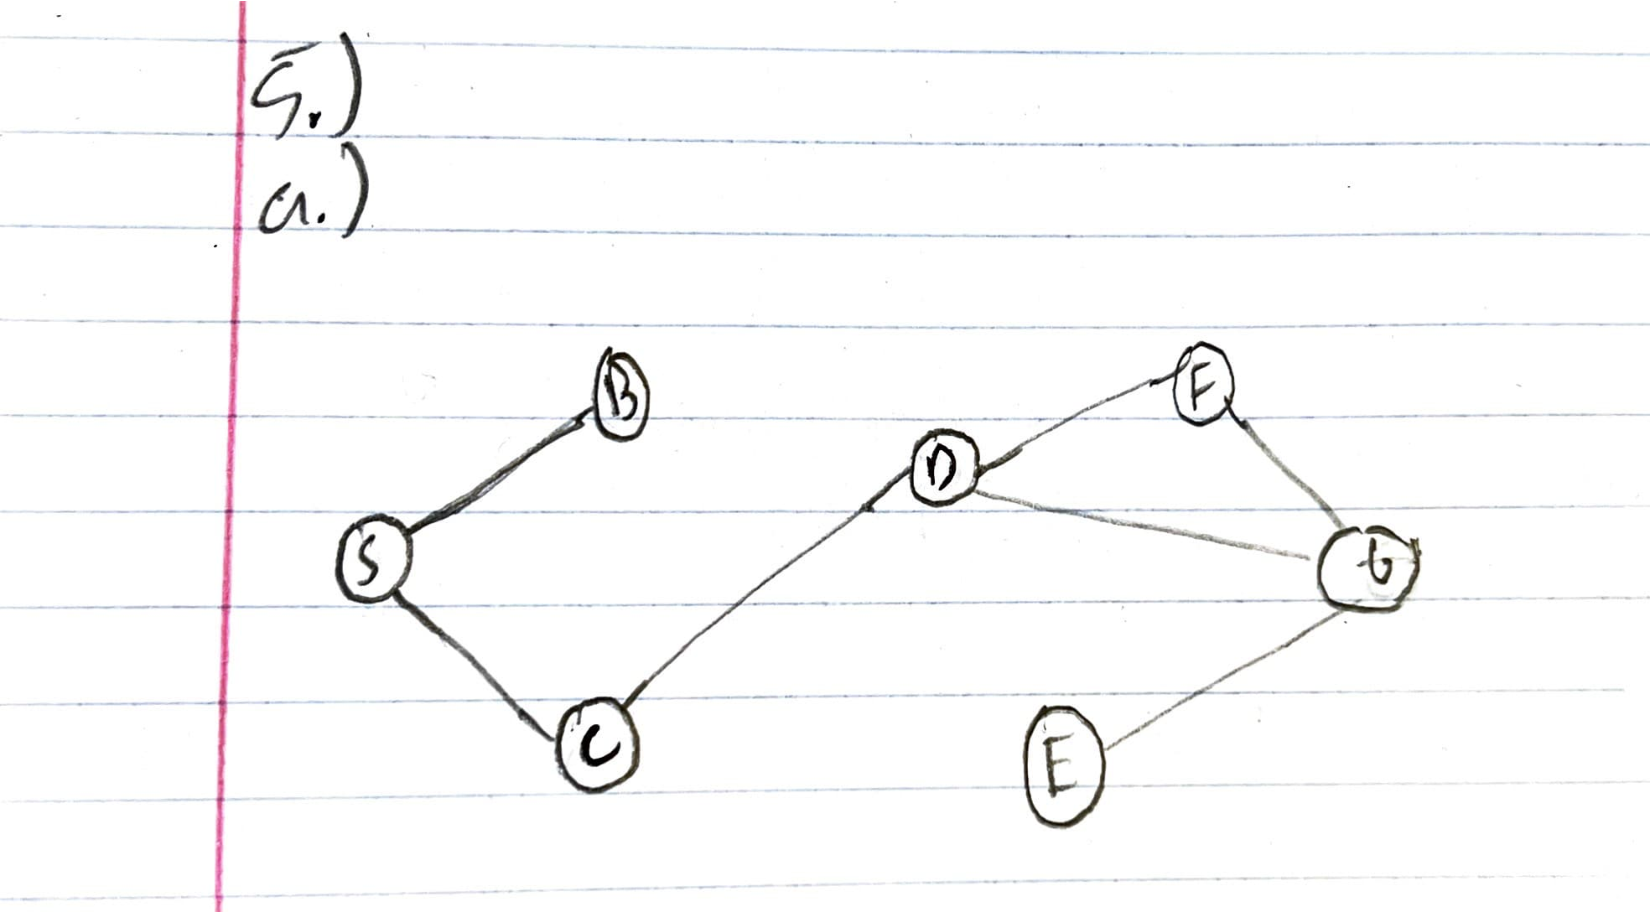
\includegraphics[width=0.5\textwidth,angle=360]{CSCI3104_HW1_Q5_A.pdf} \\
\textbf{B:} \\
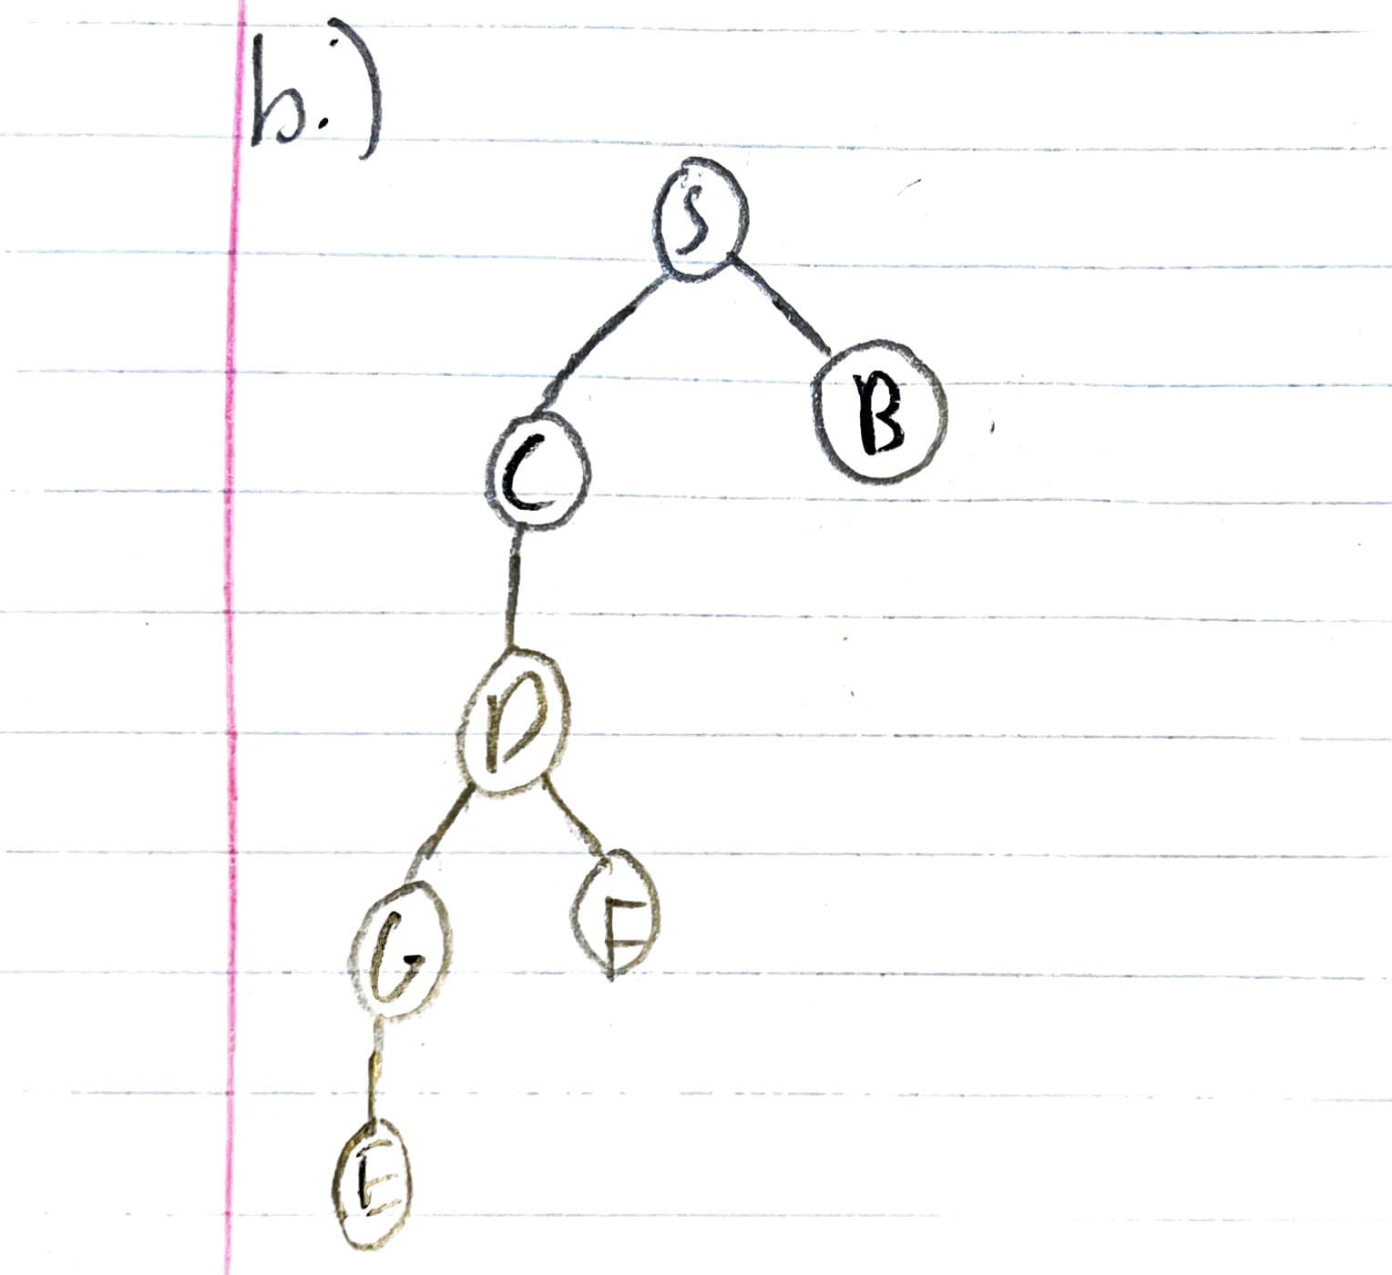
\includegraphics[width=0.5\textwidth,angle=360]{CSCI3104_Huynh_HW1_Q5B.pdf} \\

\textbf{C:} \\
The breadth-first-search algorithm that we had from class will never produce T for any ordering of the vertices because the BFS algorithm in order for it to work, the graph must be connected for all vertices regardless of the ordering. Take for example: \\
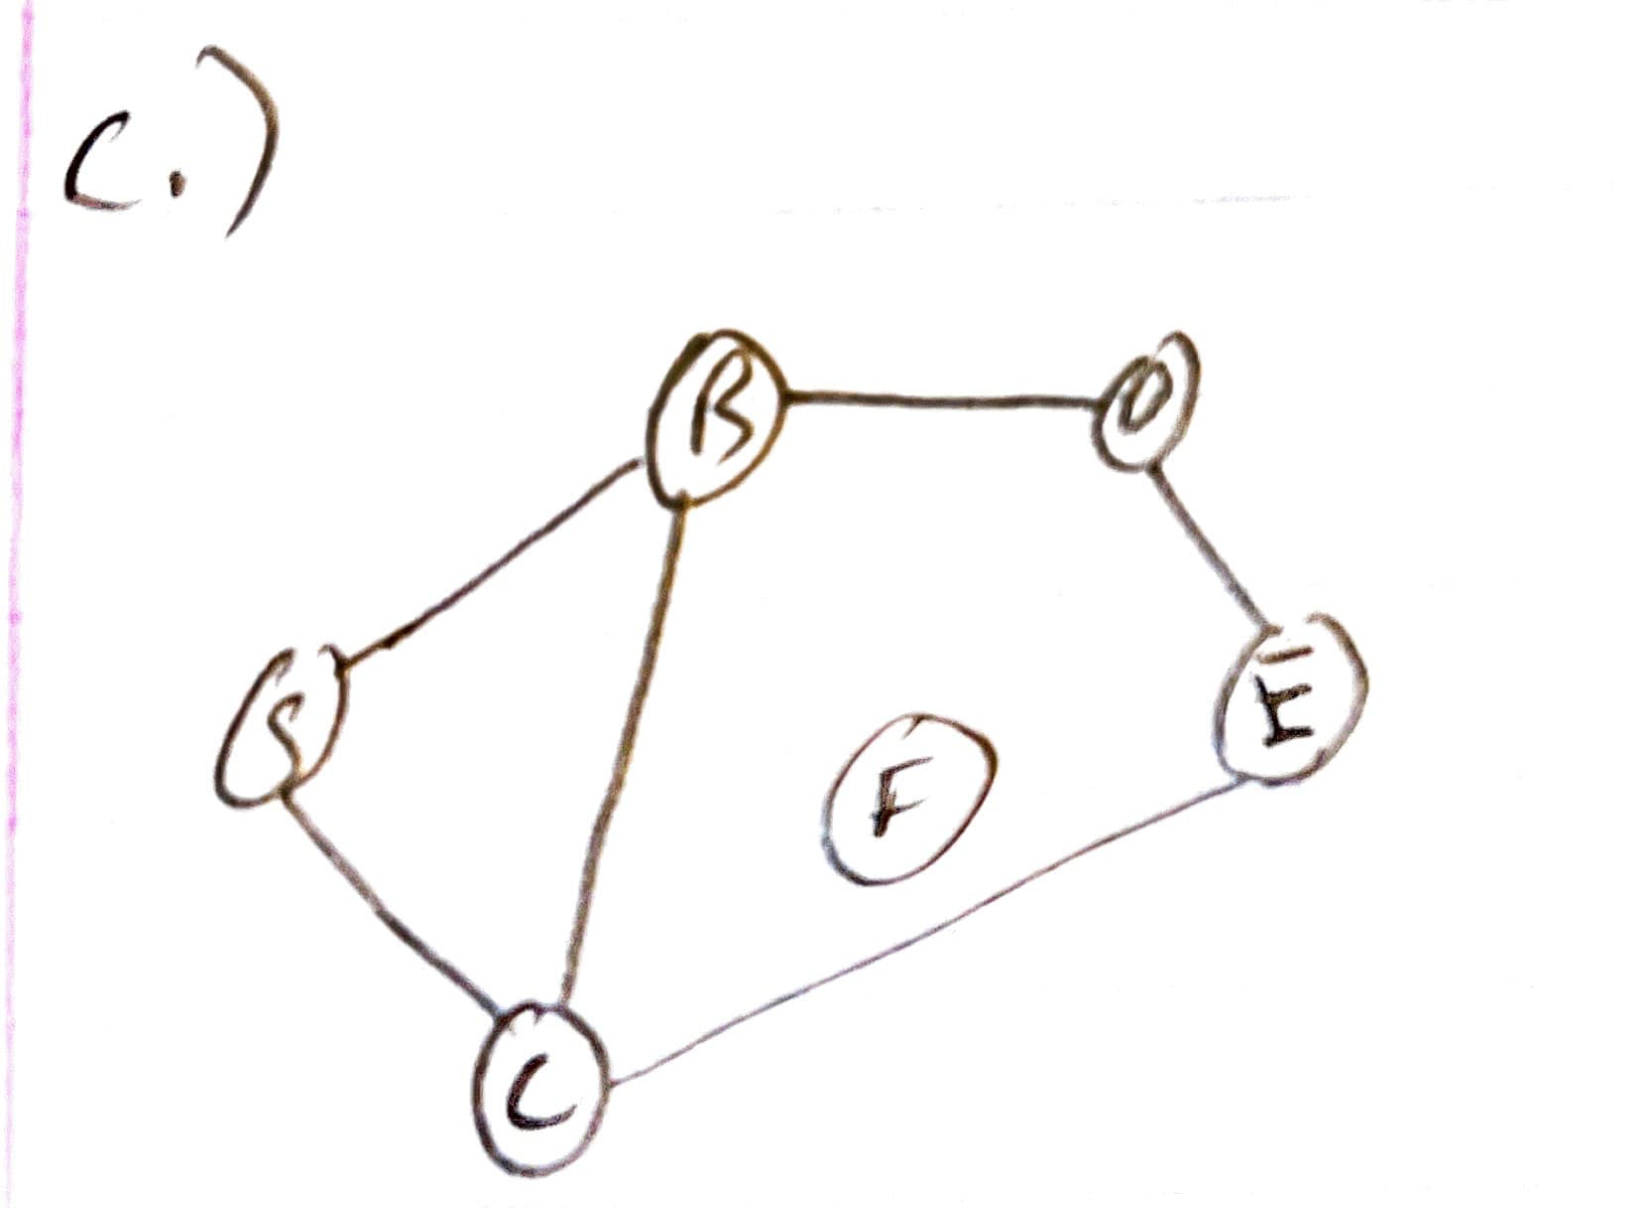
\includegraphics[width=0.5\textwidth,angle=360]{CSCI3104_HW1_Q5C.pdf} \\
Within this graph we can see that the vertex F will never be reached from the BFS algorithm because F is not connected to the rest of the graph. If we were to create a SSSPT from the BFS algorithm starting from vertex s, F would never be included within that traversal. This violates the definition of the SSSPT, as by definition,  the SSSPT must include all vertices  $V$, where $V$ is all the vertices in graph $G$, regardless of ordering. Thus, the BFS algorithm from class in this case will never be able to reproduce $T$ for any orderings of vertices because it will never visit a vertex that is not connected to the graph.



\end{proof}








\newpage
\subsection{Problem \ref{DFS4}}
\begin{required} \label{DFS4}
	Give an example of a simple, undirected, weighted graph such that a breadth-first traversal outputs a search-tree that is not a single source shortest path tree. (That is, BFS is not sufficiently powerful to solve the shortest-path problem on weighted graphs. This motivates Dijkstra's algorithm, which will be discussed in the near future.) 
	Your answer must
	\begin{enumerate}[label=(\alph*)]
		\item Draw the graph $G = (V,E, w)$ by specifying $V$ and $E$, clearly labeling the edge weights.  [\textbf{Note:} We have provided TikZ code below if you wish to use \LaTeX \ to draw the graph. Alternatively, you may hand-draw $G$ and embed it as an image below, provided that (i) your drawing is legible and (ii) we do not have to rotate our screens to grade your work.]
		\item Specify a spanning tree $T(V, E_{T})$ that is returned by BFS, but is not a single-source shortest path tree. [\textbf{Note:} You may again hand-draw this tree. If you wish, you may clearly mark the edges of $T$ on your drawing of $G$. Please make it easy on the graders to identify the edges of $T$.] 

		\item Specify a valid single-source shortest path tree $T^{\prime} = (V,E_{T^{\prime}})$.  [\textbf{Note:} You may again hand-draw this tree. If you wish, you may clearly mark the edges of $T$ on your drawing of $G$. Please make it easy on the graders to identify the edges of $T$.] 

		\item Include a clear explanation of why the search-tree output by breadth-first search is not a valid single-source shortest path tree of $G$.
	\end{enumerate}
\end{required}


\begin{proof}[Answer] Referenced Michael Levet notes, link: $https://michaellevet.github.io/Algorithms_Notes.pdf$ \\
\textbf{A:}\\
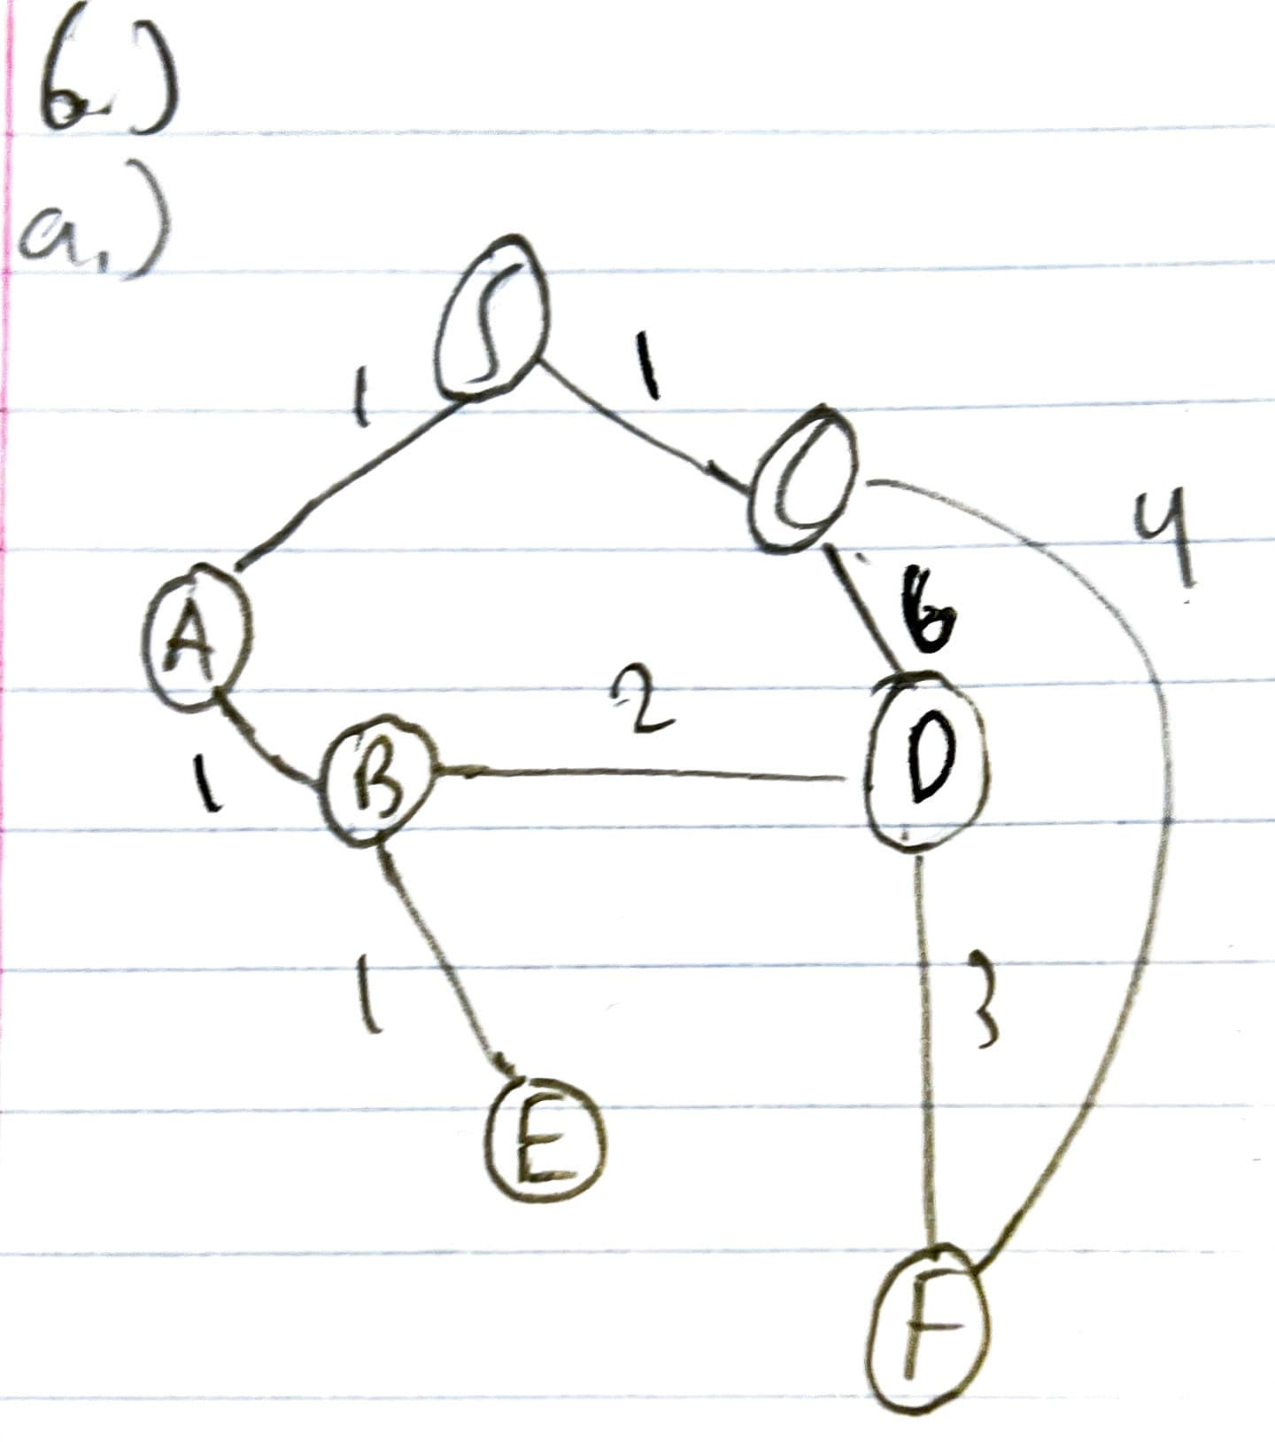
\includegraphics[width=0.5\textwidth,angle=360]{CSCI3104_HE1__Q6A.pdf} \\
\textbf{B:}\\
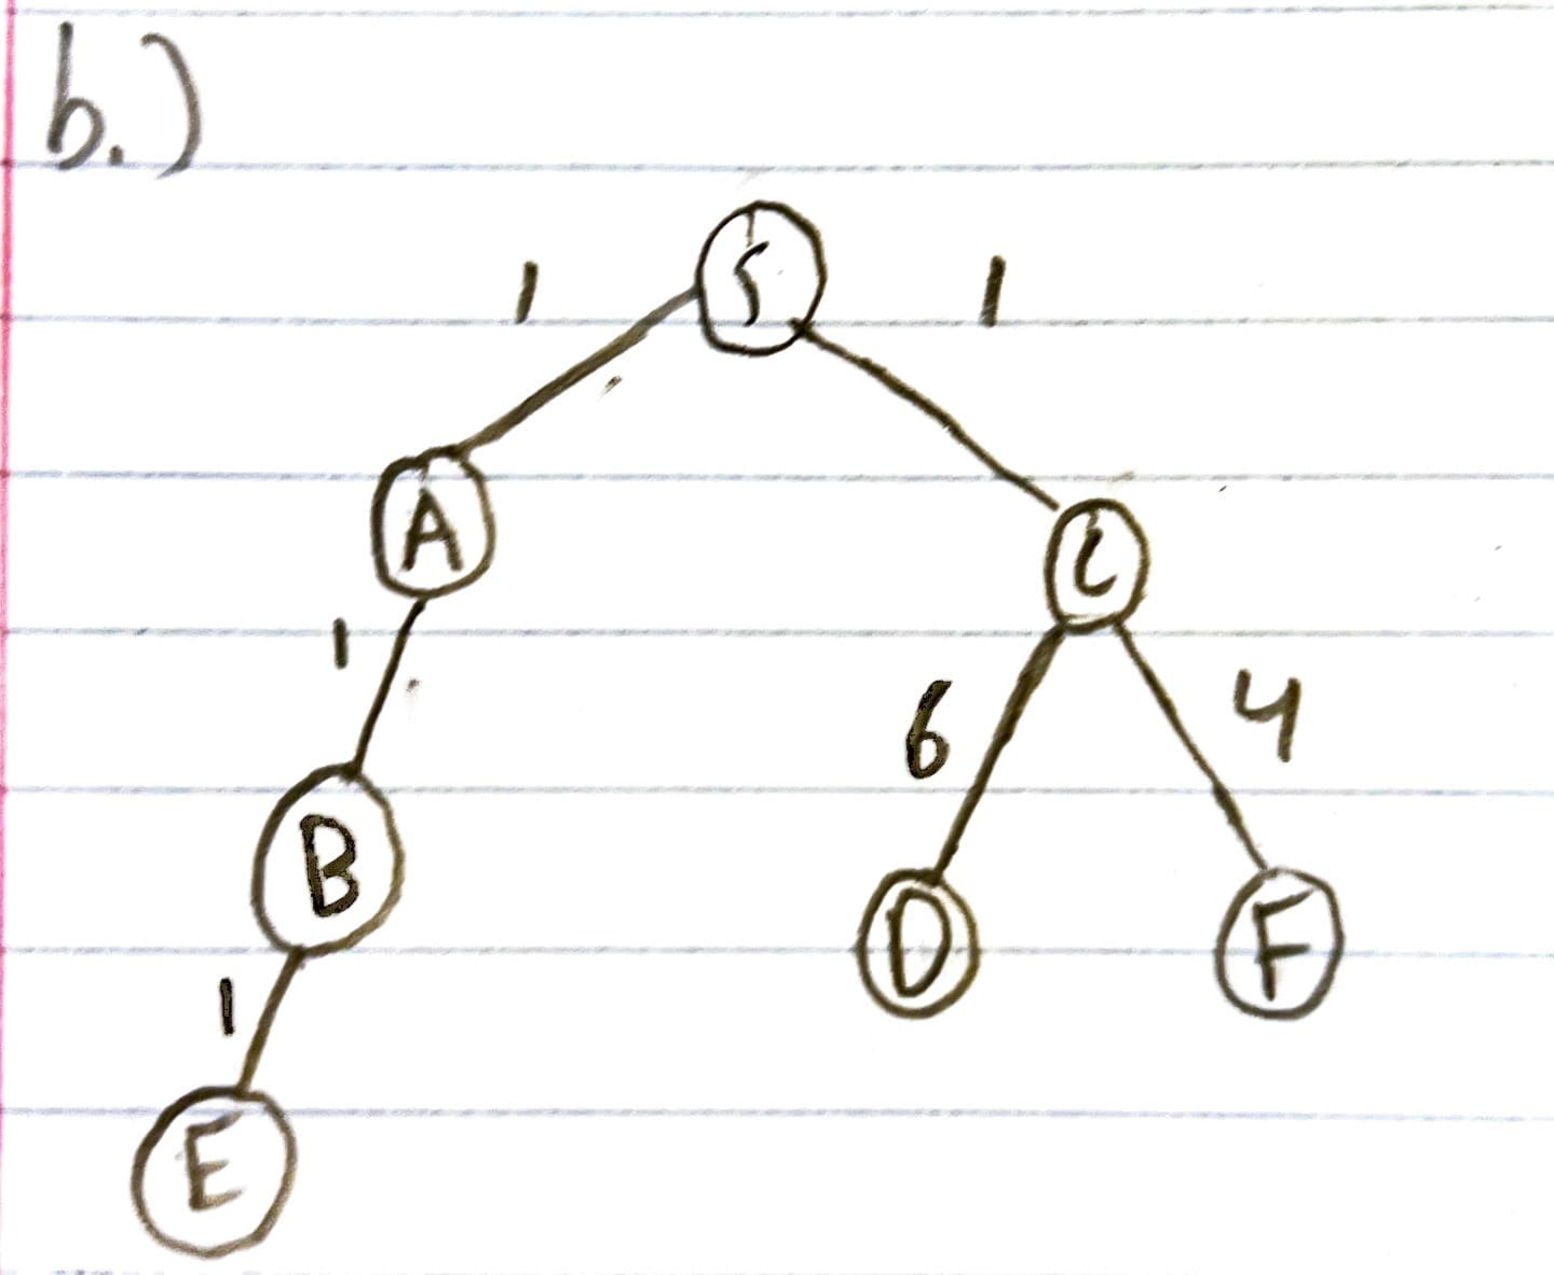
\includegraphics[width=0.5\textwidth,angle=360]{CSCI3104_HW1_Q6B.pdf} \\
\textbf{C:}\\
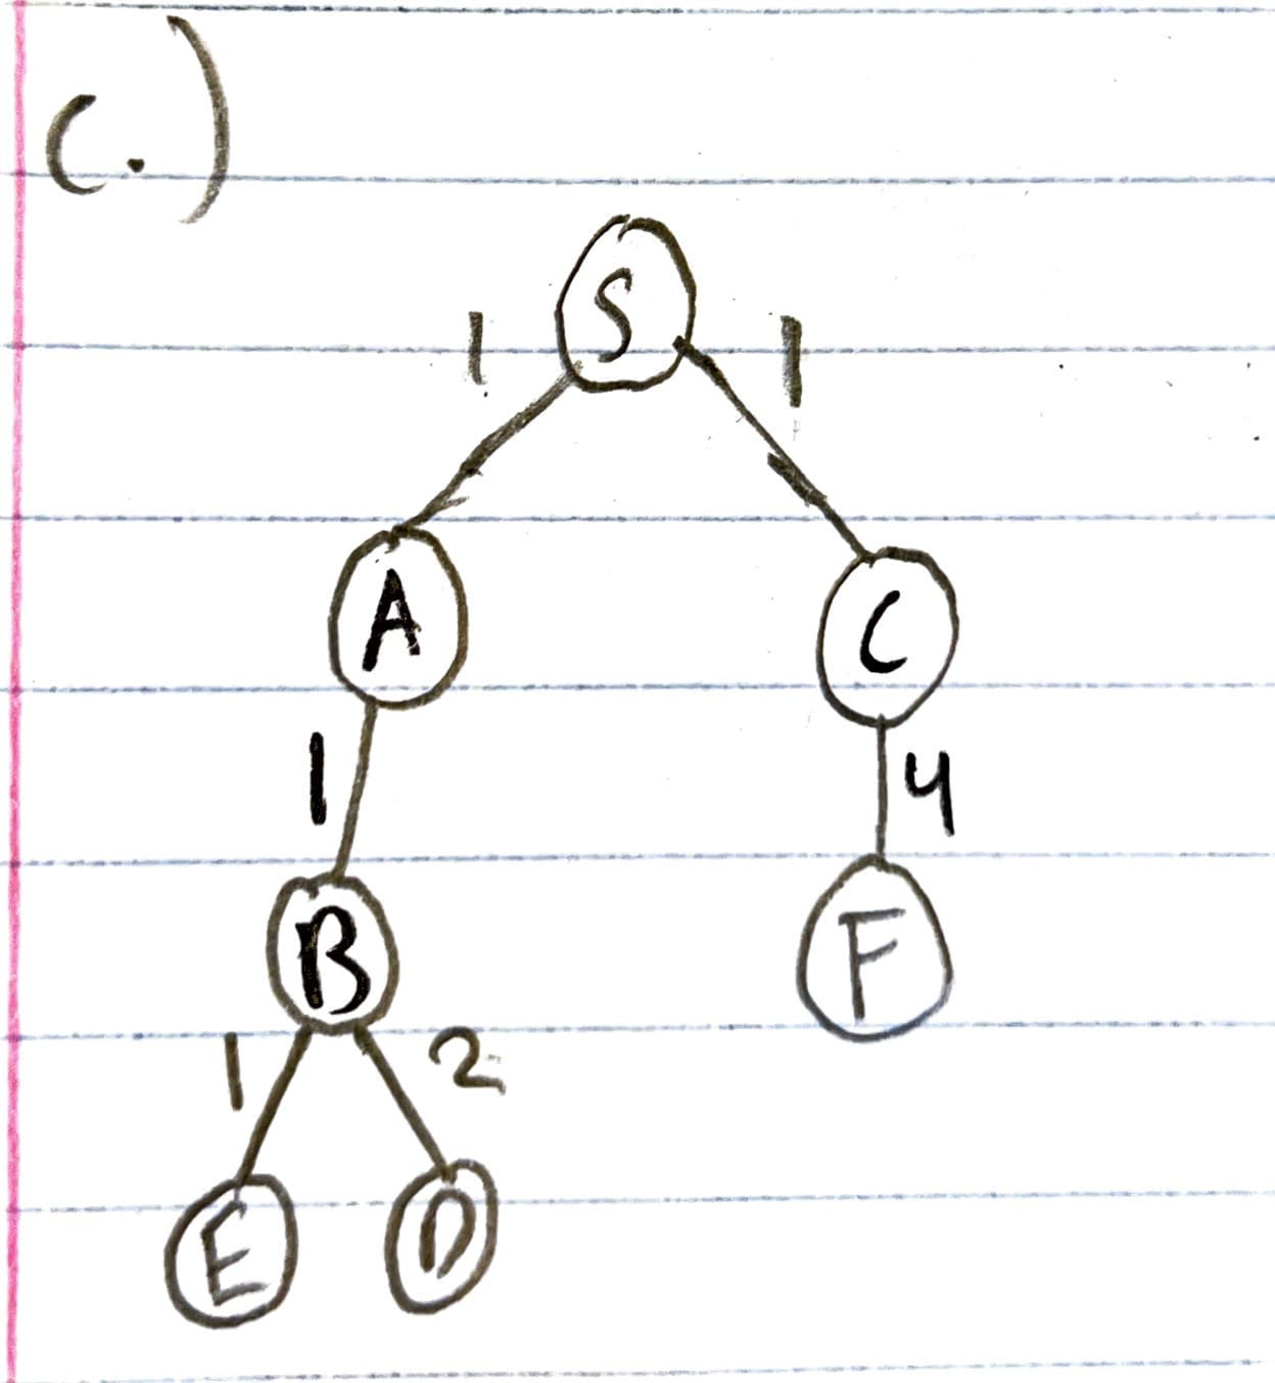
\includegraphics[width=0.5\textwidth,angle=360]{CSCI3104_HW1_Q6C.pdf} \\
\textbf {D:}\\
The breadth-first search output is not a valid single-source shortest path tree of G because it does not consider weights on each edge when the algorithm is ran. BFS when ran on a graph will treat each edge weights as equal, thus only working for unweighted graphs. Dijkstra’s algorithm when ran on a graph will account for edge weight and will further prioritize that weight, thus finding the shortest path when given a weighted graph.
\end{proof}


\end{document} % NOTHING AFTER THIS LINE IS PART OF THE DOCUMENT



